% !TEX TS-program = XeLaTeX
% use the following command:
% all document files must be coded in UTF-8
\documentclass[portuguese]{textolivre}
% build HTML with: make4ht -e build.lua -c textolivre.cfg -x -u article "fn-in,svg,pic-align"

\journalname{Texto Livre}
\thevolume{18}
%\thenumber{1} % old template
\theyear{2025}
\receiveddate{\DTMdisplaydate{2025}{5}{8}{-1}} % YYYY MM DD
\accepteddate{\DTMdisplaydate{2025}{7}{5}{-1}}
\publisheddate{\DTMdisplaydate{2025}{9}{22}{-1}}
\corrauthor{Pedro Jerónimo}
\articledoi{10.1590/1983-3652.2025.59031pt}
%\articleid{NNNN} % if the article ID is not the last 5 numbers of its DOI, provide it using \articleid{} commmand 
% list of available sesscions in the journal: articles, dossier, reports, essays, reviews, interviews, editorial
\articlesessionname{articles}
\runningauthor{Jerónimo e Torre} 
%\editorname{Leonardo Araújo} % old template
\sectioneditorname{Daniervelin Pereira}
\layouteditorname{Saula Cecília}

\title{Jornalismo local na era digital: revisão sistemática de uma década de pesquisa}
\othertitle{Local journalism in the digital age: a systematic review of a decade of research}
% if there is a third language title, add here:
%\othertitle{Artikelvorlage zur Einreichung beim Texto Livre Journal}

\author[1]{Pedro Jerónimo~\orcid{0000-0003-1900-5031}\thanks{Email: \href{mailto:pj@ubi.pt}{pj@ubi.pt}}}
\author[1]{Luisa Torre~\orcid{0000-0002-5948-106X}\thanks{Email: \href{mailto:luisa.torre@ubi.pt}{luisa.torre@ubi.pt}}}
\affil[1]{Universidade da Beira Interior, Faculdade de Artes e Letras, Departamento de Comunicação, Filosofia e Política, LabCom - Laboratório de Comunicação, Covilhã, Portugal.}


\addbibresource{article.bib}
% use biber instead of bibtex
% $ biber article

% used to create dummy text for the template file
\definecolor{dark-gray}{gray}{0.35} % color used to display dummy texts
\usepackage{lipsum}
\SetLipsumParListSurrounders{\colorlet{oldcolor}{.}\color{dark-gray}}{\color{oldcolor}}

% used here only to provide the XeLaTeX and BibTeX logos
\usepackage{hologo}

% if you use multirows in a table, include the multirow package
\usepackage{multirow}

% provides sidewaysfigure environment
\usepackage{rotating}

% CUSTOM EPIGRAPH - BEGIN 
%%% https://tex.stackexchange.com/questions/193178/specific-epigraph-style
\usepackage{epigraph}
\renewcommand\textflush{flushright}
\makeatletter
\newlength\epitextskip
\pretocmd{\@epitext}{\em}{}{}
\apptocmd{\@epitext}{\em}{}{}
\patchcmd{\epigraph}{\@epitext{#1}\\}{\@epitext{#1}\\[\epitextskip]}{}{}
\makeatother
\setlength\epigraphrule{0pt}
\setlength\epitextskip{0.5ex}
\setlength\epigraphwidth{.7\textwidth}
% CUSTOM EPIGRAPH - END

% to use IPA symbols in unicode add
%\usepackage{fontspec}
%\newfontfamily\ipafont{CMU Serif}
%\newcommand{\ipa}[1]{{\ipafont #1}}
% and in the text you may use the \ipa{...} command passing the symbols in unicode

% LANGUAGE - BEGIN
% ARABIC
% for languages that use special fonts, you must provide the typeface that will be used
% \setotherlanguage{arabic}
% \newfontfamily\arabicfont[Script=Arabic]{Amiri}
% \newfontfamily\arabicfontsf[Script=Arabic]{Amiri}
% \newfontfamily\arabicfonttt[Script=Arabic]{Amiri}
%
% in the article, to add arabic text use: \textlang{arabic}{ ... }
%
% RUSSIAN
% for russian text we also need to define fonts with support for Cyrillic script
% \usepackage{fontspec}
% \setotherlanguage{russian}
% \newfontfamily\cyrillicfont{Times New Roman}
% \newfontfamily\cyrillicfontsf{Times New Roman}[Script=Cyrillic]
% \newfontfamily\cyrillicfonttt{Times New Roman}[Script=Cyrillic]
%
% in the text use \begin{russian} ... \end{russian}
% LANGUAGE - END

% EMOJIS - BEGIN
% to use emoticons in your manuscript
% https://stackoverflow.com/questions/190145/how-to-insert-emoticons-in-latex/57076064
% using font Symbola, which has full support
% the font may be downloaded at:
% https://dn-works.com/ufas/
% add to preamble:
% \newfontfamily\Symbola{Symbola}
% in the text use:
% {\Symbola }
% EMOJIS - END

% LABEL REFERENCE TO DESCRIPTIVE LIST - BEGIN
% reference itens in a descriptive list using their labels instead of numbers
% insert the code below in the preambule:
%\makeatletter
%\let\orgdescriptionlabel\descriptionlabel
%\renewcommand*{\descriptionlabel}[1]{%
%  \let\orglabel\label
%  \let\label\@gobble
%  \phantomsection
%  \edef\@currentlabel{#1\unskip}%
%  \let\label\orglabel
%  \orgdescriptionlabel{#1}%
%}
%\makeatother
%
% in your document, use as illustraded here:
%\begin{description}
%  \item[first\label{itm1}] this is only an example;
%  % ...  add more items
%\end{description}
% LABEL REFERENCE TO DESCRIPTIVE LIST - END


% add line numbers for submission
%\usepackage{lineno}
%\linenumbers

\begin{document}
\maketitle

\begin{polyabstract}
\begin{abstract}
Este artigo sintetiza a pesquisa sobre jornalismo local digital realizada entre 2013 e 2023. Mediante uma revisão sistemática da literatura (n=149), foram identificados seis agrupamentos de pesquisa: práticas jornalísticas, panoramas mediáticos, transformação digital, envolvimento da audiência, modelos de negócio e participação cívica. Os resultados enfatizam o duplo desafio da inovação e sustentabilidade, especialmente para os media menores e em contextos de escassez de recursos, enquanto o jornalismo local continua a desempenhar um papel fundamental na identidade das comunidades, apesar de o seu futuro ser ameaçado por desertos de notícias, vieses algorítmicos e déficits de financiamento. Também sublinham a intrínseca ligação entre a inovação tecnológica, a sustentabilidade dos modelos de negócio e o fomento da participação cívica, essenciais para a resiliência do jornalismo local. A pesquisa permanece concentrada no Norte Global, apontando para a necessidade de uma representação geográfica mais ampla. Sugerem-se futuros estudos que abordem o uso ético de Inteligência Artificial, a resiliência hiperlocal e mecanismos de construção de confiança.

\keywords{Jornalismo local\sep Jornalismo digital\sep Produção de notícias\sep Media locais\sep Revisão sistemática}
\end{abstract}

\begin{english}
\begin{abstract}
This paper summarizes research on digital local journalism conducted between 2013 and 2023. Through a systematic literature review (n=149), six research clusters were identified: journalistic practices, media landscapes, digital transformation, audience engagement, business models, and civic participation. The findings highlight the dual challenges of innovation and sustainability, especially for smaller media outlets in resource-scarce contexts. Local journalism continues to play a key role in community identity, despite threats to its future posed by the spread of news deserts, the dangers of algorithmic biases and funding difficulties. These results also stress the intrinsic connection between technological innovation, business model sustainability, and the fostering of civic participation, all of which are essential to the resilience of local journalism. Research remains concentrated in the Global North, pointing to the need for broader geographical representation. Future studies are suggested regarding the ethical use of Artificial Intelligence, hyperlocal resilience, and mechanisms for building trust.

\keywords{Local journalism\sep Digital journalism\sep News production\sep Local media\sep Systematic review}
\end{abstract}
\end{english}
% if there is another abstract, insert it here using the same scheme
\end{polyabstract}

\section{Introdução}

Trinta anos após a internet se tornar central nas redações, novos desafios emergem. As redes sociais e os motores de pesquisa transformaram a forma como as notícias são distribuídas, os modelos de negócios tradicionais tornaram-se cada vez mais inviáveis, a proliferação de desinformação intensificou-se numa crise significativa, e os mais recentes avanços em Inteligência Artificial (IA) trouxeram novas complexidades.

As primeiras pesquisas sobre jornalismo digital centraram-se na distribuição e no produto, seguidas por uma abordagem etnográfica \cite{jeronimo2015}. As transformações nas condições de trabalho também foram consideradas \cite{deuze2009, morais2020}. Estudos recentes têm-se concentrado na tecnologia, plataformas e audiências \cite{steensen2019}, explorando como o “digital” afeta e é afetado pelo jornalismo na sociedade. A pesquisa em jornalismo digital posiciona-se entre a continuidade e a mudança. Analisa a crise que os media enfrentam, os processos de inovação e adaptação do jornalismo, e a crescente diluição das fronteiras entre jornalistas e audiências, fatos e opiniões, e notícias reais e falsas \cite{eldridge2019, westlund2023}.

Os académicos têm empregado diversas terminologias para referir ao jornalismo digital, com as comunidades de língua inglesa e latino-americana a preferirem “jornalismo online” ou “jornalismo digital” \cite{boczkowski2004, westlund2023, eldridge2019}, enquanto as de língua portuguesa e espanhola utilizam “ciberjornalismo” \cite{bastos2023, jeronimo2015, diaz2003, lopez-garcia2008}. Apesar de termos como “online” e “jornalismo multimédia” terem dominado os primeiros estudos, “jornalismo digital” ganhou destaque após 2010 com o lançamento da revista Digital Journalism em 2013 \cite{steensen2019}. Independentemente da terminologia, todos se referem ao jornalismo disseminado online, mesmo quando se trata de notícias locais \cite{jeronimo2015}.

O jornalismo digital é agora uma “disciplina estabelecida”. No entanto, ainda existem alguns desafios, incluindo um maior foco nos media nativos ou exclusivamente digitais, à realização de pesquisas orientadas para a inovação, e uma maior atenção a tópicos e áreas que recebem pouca atenção \cite{salaverria2019}, uma perspetiva em que o jornalismo local se encontra e que este artigo visa abordar. A estreita relação entre media locais e audiências permite que os jornalistas desenvolvam processos específicos de definição de agenda, devido aos laços mais estreitos com o público que desejam informar \cite{correia2019fake}. Assim, as notícias locais são resultado de um jornalismo comprometido com o território e com as pessoas que a ele se relaciona, geograficamente ou emocionalmente – comunidades em que o jornalista partilha os mesmos valores culturais e espaços sociais e, muitas vezes, também faz parte \cite{camponez2002, lopez-garcia2008}. Partilhar as mesmas comunidades permite aos jornalistas ter um conhecimento mais profundo sobre os fatos que cobrem, mas esta proximidade pode resultar na falta de independência e distância que a deontologia jornalística pede \cite{jeronimo2015}. Estes meios de comunicação desempenham um papel fundamental no atendimento das necessidades informativas das comunidades locais, enquanto têm a capacidade de moldar a forma como os membros da comunidade se percebem e as suas realidades locais \cite{nielsen2015}.

O jornalismo mudou ao perder a centralidade da produção e disseminação de informação, algo que também o público passou a poder fazer \cite{castells2015}. Surge o gatekeeping algorítmico, um mecanismo relevante de visibilidade das notícias e disseminação de desinformação \cite{cardoso2023}. As grandes empresas tecnológicas passaram a absorver a maior parte das receitas de publicidade que costumavam sustentar o negócio dos media, particularmente os locais \cite{costa2014}. Os jornalistas enfrentam um ambiente de trabalho cada vez mais acelerado, marcado pela procura pela inovação tecnológica e que altera as tarefas e a organização das redações. A integração da automação e da IA afeta a produção, distribuição e recepção das notícias, também em redações menores \cite{goncalves2024}. Num mundo em mudança, que também implica o trabalho dos jornalistas locais, quais são os temas e desafios que emergem da pesquisa realizada no período de 2013-2023?

Revisões recentes da literatura sobre jornalismo local centraram-se nos media hiperlocais \cite{negreira-rey2021, negreira-rey_amigo2022}, nos desertos de notícias \cite{rodriguezurra2024} e na erosão da proximidade no jornalismo local \cite{mota2023}. Porém, estudos sobre o jornalismo digital numa escala local – ou ciberjornalismo de proximidade, como defendem outros autores \cite{lopez-garcia2008, jeronimo2015} – permanecem um tópico a ser melhor explorado, especialmente perante os desafios face à desinformação, ao uso de redes sociais e ao impacto da plataformização \cite{poell2020plataformizacao, morais2023}. Este artigo explora as mudanças no jornalismo local digital, destacando desafios tecnológicos, impactos nas democracias e dinâmicas de informação em pequenas comunidades. Esta observação relaciona-se com o papel da informação jornalística local na identidade e coesão comunitária. Ao conectar pessoas em espaços digitais e físicos através de valores sociais e culturais partilhados, atua como uma 'cola social' que constrói um sentimento de comunidade \cite{hess2015}.

O período estudado (2013-2023) fica marcado pelo rápido crescimento na digitalização e pelas profundas mudanças na interação dos media com as audiências \cite{heiselberg2024}. Pretendemos investigar se o interesse da pesquisa cresceu ao longo dos anos e se as revistas mais relevantes estão a dedicar espaço a este tema, para compreender a sua relevância dentro do campo mais amplo dos estudos de jornalismo digital. Também pretendemos compreender quais os principais tópicos investigados, para perceber se a pesquisa sobre jornalismo digital que é local também evoluiu para um maior foco em tecnologia, plataformas e audiências, como se verificou para o jornalismo digital \cite{steensen2019}, ou se existem temas particulares ligados a uma abordagem mais local. Além disso, observar quais os países mais pesquisados, para analisar se existem países ou regiões sub-estudadas e que poderiam beneficiar de pesquisas futuras, ou se existem algumas preferências temáticas dentro de algumas regiões. Por meio de uma revisão sistemática da literatura sobre jornalismo local digital, pretendemos analisar e compreender a pesquisa realizada ao longo de 10 anos neste campo. Com base neste panorama e nas lacunas identificadas, colocamos as seguintes questões:

\begin{itemize}
    \item RQ1. Quais são os temas e metodologias adotados na pesquisa sobre jornalismo digital local na última década (2013-2023) e como é que eles refletem os desafios e transformações no campo?
    \item RQ2. Quais são os contextos geográficos mais frequentemente abordados, em que revistas e como é que esses padrões influenciam a compreensão do jornalismo digital local globalmente? 
\end{itemize}



\section{Material e métodos}

Este estudo foi conduzido como uma revisão sistemática da literatura, com o objetivo de mapear e analisar a pesquisa sobre jornalismo local digital. A metodologia adotada priorizou a transparência e a replicabilidade, focando-se em publicações científicas para garantir a qualidade dos dados. A escolha de textos publicados exclusivamente em inglês justifica-se pela prevalência e impacto da produção académica nessa língua nas bases de dados internacionais de comunicação, permitindo uma análise focada na literatura de maior alcance global no período definido (2013-2023). A extração de dados foi realizada através da base de dados Scopus, reconhecida pela sua abrangência em periódicos científicos, garantindo uma cobertura relevante para a área. A análise dos dados procedeu em duas etapas principais: inicialmente, uma abordagem quantitativa para identificar tendências numéricas (como ano de publicação, periódicos e afiliações), seguida de uma análise qualitativa aprofundada para categorizar e discutir os temas e metodologias predominantes. Esta estrutura visa proporcionar uma compreensão clara das tendências e lacunas da pesquisa.

A extração de dados ocorreu entre setembro e outubro de 2024 e os critérios de inclusão incluíram publicações que se focassem no jornalismo local digital, que tivessem uma boa correspondência com as palavras-chave e categorias escolhidas (“Ciências Sociais” e “Artes e Humanidades”), que estivessem dentro do período proposto e que fossem publicadas em inglês. Os critérios de exclusão incluíram resultados duplicados para as palavras-chave selecionadas, tópicos não correspondentes e um foco em enquadramentos muito específicos ao analisar os media locais, bem como não discutir o jornalismo local digital.

Um total de 18 combinações de palavras-chave foram pesquisadas, resultando em 1.529 entradas. Destas, 692 referências foram excluídas por serem duplicadas e considerando a melhor correspondência com as palavras-chave, restando 837 entradas. A pesquisa de palavras-chave incluiu combinações entre as palavras “digital”, “e” ou “e”; “local” e “proximidade”; “jornalismo”, “jornalistas” e “notícias”. Em seguida, foram lidos os resumos das publicações e, em alguns casos, uma leitura superficial da publicação.

Os critérios de exclusão incluem: artigos que não fossem em inglês; resumo indisponível online; artigos que se referiam amplamente a jornalismo local ou notícias locais, mas sem foco no digital. Trabalhos que se concentravam noutros tópicos relacionados ao jornalismo local (por exemplo, media de serviço público ou media étnica), mas não se focavam no digital, não foram incluídos. Pesquisas sobre audiências de notícias locais que não separavam as audiências de notícias digitais das audiências offline não foram consideradas. Temas estreitamente ligados ao jornalismo local (por exemplo, hiperlocal, jornalismo cidadão, jornalismo comunitário, “desertos de notícias”), que falavam sobre organizações de notícias digitais ou jornalistas, foram incluídos e agregados em agrupamentos temáticos. Publicações que incluíram análises sobre jornalismo local online juntamente com órgãos de comunicação locais tradicionais/estabelecidos offline (comparações, etc.) também foram incluídas na amostra. A aplicação sistemática dos critérios de exclusão resultou na remoção de 688 publicações, uma das quais não tinha resumo, restando uma amostra final de 149 publicações (ver \Cref{tab-1}).


%--- código da tabela 1 ---%
\begin{table}[h!]
\centering
\begin{threeparttable}
\caption{Resultado das buscas por palavras-chave.}\label{tab-1}
\begin{tabular}{lccc}
\toprule
Keywords & Excluído & Incluído & Total \\
\midrule
digital + local + journalism & 199 & 3  & 202 \\
digital + local + journalists & 94 & 13 & 107 \\
digital + local + news & 269 & 46 & 315 \\
digital + proximity + journalism & 20 & 0 & 20 \\
digital + proximity + journalists & 16 & 0 & 16 \\
digital + proximity + news & 23 & 3 & 26 \\
online + local + journalism & 136 & 53 & 189 \\
online + local + journalists & 128 & 10 & 138 \\
online + local + news & 439 & 19 & 458 \\
online + proximity + journalism & 9 & 0 & 9 \\
online + proximity + journalists & 5 & 0 & 5 \\
online + proximity + news & 35 & 2 & 37 \\
cyber + local + news & 5 & 0 & 5 \\
cyber + local + journalism & 0 & 0 & 0 \\
cyber + local + journalists & 0 & 0 & 0 \\
cyber + proximity + journalism & 0 & 0 & 0 \\
cyber + proximity + journalists & 0 & 0 & 0 \\
cyber + proximity + news & 2 & 0 & 2 \\
\addlinespace[0.3em]
Total & 1.380 & 149 & 1.529 \\
\bottomrule
\end{tabular}
\source{Elaboração própria.}
\end{threeparttable}
\end{table}

A seleção foi manual e o processo de codificação foi partilhado pelos dois autores deste estudo: um investigador realizou a codificação e o outro a reviu. Os desacordos foram discutidos. O processo consistiu em três etapas. Iniciou-se com a exploração do material e a revisão da literatura, o que levou à delimitação das categorias de análise propostas. O objetivo foi sistematizar ideias para desenvolver um esquema de operações sucessivas \cite{bardin1977}. Após a pré-análise, procedeu-se à fase de codificação, que consistiu em três fases: recorte da unidade de codificação, escolha da regra de enumeração e escolha das categorias. Observou-se a amostra em relação a tópicos, abordagens e metodologias do jornalismo local digital. Ao analisar a base de dados, enumeraram-se as seguintes características técnicas: (1) Ano de publicação; (2) Nome do periódico/livro/conferência; (3) Autores; (4) Afiliação; (5) Tipo de publicação. Ao analisar os resumos, observou-se: (1) tema principal, que posteriormente foi agregado em agrupamentos maiores; (2) quais as metodologias aplicadas ao estudo; (3) o contexto geográfico abordado. Para o tema principal, as categorias desenvolvidas foram: digital; pesquisa de audiência; modelos de negócio; panorama dos media locais; envolvimento cívico; prática e papéis jornalísticos. Em todos os casos, observou-se o ângulo principal adotado pelos pesquisadores para inseri-lo nas categorias.

\section{Resultados}

\subsection{Análise de características técnicas e tendências de pesquisa}

%--- código da figura 1 ---%
\begin{figure}[htbp]
\centering
\begin{minipage}{0.75\textwidth}
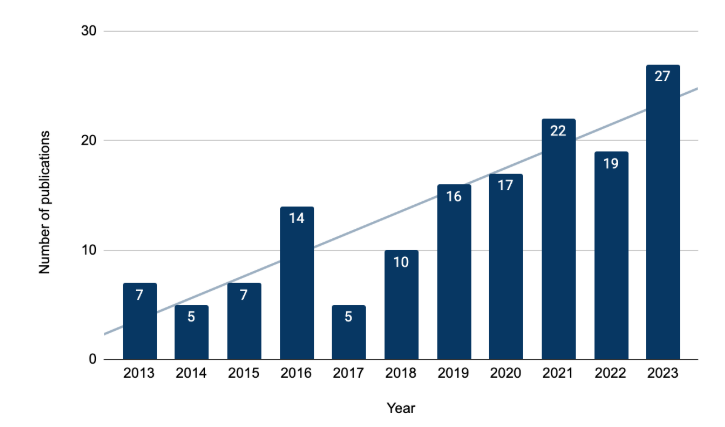
\includegraphics[width =\textwidth]{Imagens/Fig1.png}
\caption{Número de publicações sobre jornalismo local digital por ano.}
\label{fig-1}
\source{Elaboração própria.}
\end{minipage}
\end{figure}


O interesse pela pesquisa sobre jornalismo local digital cresceu ao longo do período analisado (2013-2023), com um aumento notável de publicações a partir de 2017 (\Cref{fig-1}). Nesta amostra, e sem surpresa, a revista com mais artigos publicados é o \textit{Digital Journalism} (27), seguidas pela \textit{Journalism Practice} (17), \textit{Journalism Studies} (14), \textit{Journalism} (10) e \textit{Media and Communication} (4). A amostra, no entanto, é muito fragmentada, compreendendo 61 publicações diferentes de âmbitos e realidades regionais muito diversas. Revistas que cobrem áreas geográficas específicas também são importantes nesta amostra, como a \textit{Nordicom Review} (10) e a \textit{Media International Australia} (3), o que sugere uma relação com o robusto ecossistema de notícias locais encontrado nos países nórdicos e na Austrália. Também se destaca a presença de livros, como Local \textit{Journalism: Critical Perspectives on the Provincial Newspaper}, editado por \textcite{matthews2023}, com 6 capítulos (\Cref{fig-2}).

%--- código da figura 2 ---%
\begin{figure}[htbp]
\centering
\begin{minipage}{0.70\textwidth}
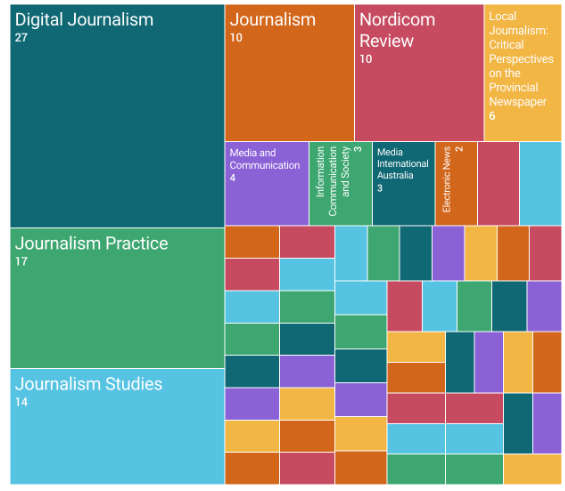
\includegraphics[width =\textwidth]{Imagens/Fig2.png}
\caption{Revistas, livros ou livros de atas com mais artigos publicados.}
\label{fig-2}
\source{Elaboração própria.}
\end{minipage}
\end{figure}

Em relação à autoria, foram encontrados 254 académicos como autores ou coautores nas publicações, o que representa menos de 2 autores em média (M=1.7) por publicação. Considerando o país de afiliação, cerca de 30\% deles (78) são de universidades e centros de pesquisa dos Estados Unidos. Académicos do Norte Global estão bem representados, com o Reino Unido (40), Suécia (25), Noruega (19) e Austrália (15) constituindo a maioria desta amostra.

A maioria das publicações analisadas são artigos (124); numa escala muito inferior estão os capítulos de livros (14), livros (5) e artigos de conferências (6) (\Cref{fig-3}).


%--- código da figura 3 ---%
\begin{figure}[htbp]
\centering
\begin{minipage}{0.85\textwidth}
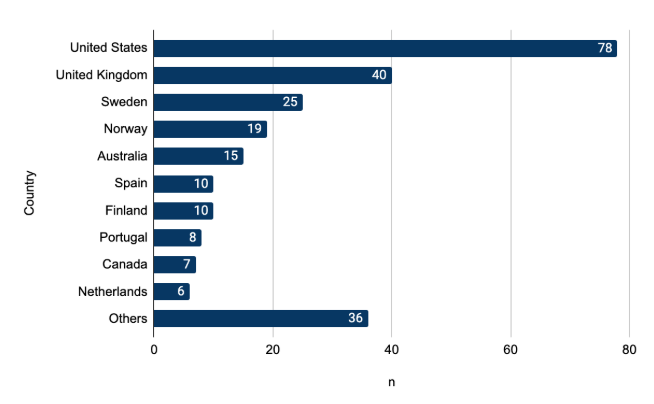
\includegraphics[width =\textwidth]{Imagens/Fig3.png}
\caption{Afiliação dos autores por países.}
\label{fig-3}
\source{Elaboração própria.}
\end{minipage}
\end{figure}

A maioria dos estudos (129) focou em um único país, 16 analisaram vários e 4 não especificaram um contexto geográfico. Os EUA foram o país mais estudado sobre jornalismo local digital (42 publicações), seguidos pelo Reino Unido (21), Noruega (17), Suécia (16), Austrália (12) e Espanha (7). Nos últimos 10 anos, a pesquisa se concentrou na Europa Ocidental, países nórdicos e América anglófona, o que provavelmente foi influenciado pela exclusão de trabalhos não escritos em inglês e pela base de dados usada (Scopus). Alguns estudos abordam realidades asiáticas e africanas, como Malásia (3), Indonésia (2), Tanzânia (1), Etiópia (1) e África do Sul (1).

A maioria dos estudos analisados é empírica (141), com poucas abordagens teóricas (8). Há um equilíbrio entre métodos qualitativos (56) e quantitativos (62), com leve predominância dos últimos. Métodos mistos também são comuns (23). Os qualitativos mais usados incluem entrevistas, grupos focais, observação e estudos de caso. Nos quantitativos, destacam-se inquéritos e análise de conteúdo. Já os métodos mistos combinam inquéritos, entrevistas, grupos focais e observação (\Cref{fig-4}).

%--- código da figura 4 ---%
\begin{figure}[htbp]
\centering
\begin{minipage}{0.70\textwidth}
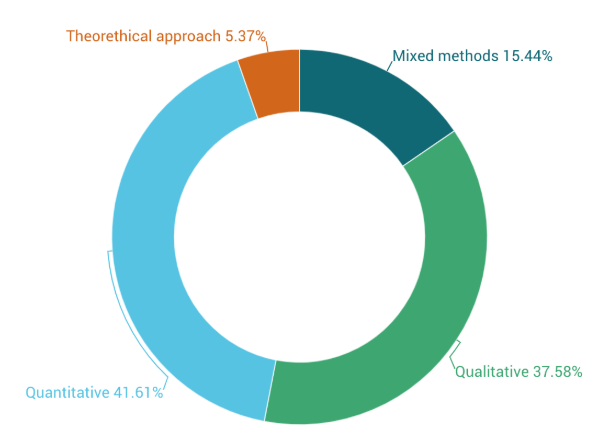
\includegraphics[width =\textwidth]{Imagens/Fig4.png}
\caption{Metodologias adotadas nos estudos analisados.}
\label{fig-4}
\source{Elaboração própria.}
\end{minipage}
\end{figure}

\subsection{Análise do conteúdo}

Os principais temas investigados podem ser agrupados em 6 categorias, identificadas a partir dos padrões temáticos dos artigos analisados pelos pesquisadores.

O primeiro agrupamento (n=31) trata da prática jornalística e dos papéis dos media locais digitais, incluindo uso de redes sociais, lacunas na cobertura e características desses meios, e será chamado Prática e Papéis Jornalísticos. O segundo (n=31) aborda o ecossistema dos media locais digitais, incluindo mapeamento e outros atores como jornalismo alternativo e comunitário, e será denominado Panorama dos Media Locais Digitais. O terceiro (n=24) foca na transformação digital, como o uso de IA, algoritmos, e a digitalização do jornalismo, sendo denominado Transformação Digital. O quarto (n=30) está relacionado à pesquisa sobre as audiências, incluindo interações nas redes sociais, jornalismo cidadão e consumo de notícias, chamado Pesquisa de Audiência. O quinto (n=24) aborda Modelos de Negócio, analisando fluxos de receita e sustentabilidade econômica dos meios locais digitais. Por fim, o agrupamento Envolvimento Cívico (n=9) investiga a relação da mídia local digital com a participação cívica e política.

Ao cruzar temas e países investigados, não foram encontrados padrões claros, mas existem algumas conclusões a destacar. Estudos que investigaram a Austrália e relacionados ao envolvimento cívico foram muito relevantes na amostra do país (5); em estudos focados na Noruega, 7 das 17 publicações investigaram o tema dos modelos de negócios; na Suécia e no Reino Unido, os hiperlocais destacam-se, com 5 e 4 estudos, respetivamente; nos EUA, a pesquisa relacionada com a prática e os papéis jornalísticos é bastante significativa (12).

\subsubsection{Prática e papéis jornalísticos nos \textit{media} locais digitais}

\subsubsubsection{Prática jornalística}

Com a digitalização das notícias, os jornalistas locais precisam adaptar suas práticas. A cultura organizacional das redações locais influencia a resposta às mudanças digitais \cite{ohara2023}. Muitos repórteres digitais ainda produzem histórias convencionais, baseadas em práticas tradicionais \cite{ryfe2016}. O jornalismo local digital na Europa sofre com superficialidade e falta de adaptação ao formato online, mas poderia se beneficiar de novas formas de conexão com o público, como narrativas transmedia \cite{rivasderoca2020}.

\subsubsubsection{Métricas e seus efeitos}
À medida que as notícias povoam o mundo digital, jornalistas e editores locais enfrentam uma nova pressão: a das métricas de tráfego, que influenciam a escolha de conteúdo e a forma como as histórias são partilhadas nas redes sociais, afetando as práticas jornalísticas nas redações e as normas do jornalismo para dispositivos móveis \cite{blanchettneheli2018, perreault2019}. Para atender a estas pressões, muitas redações perseguem a cobertura de notícias de última hora e os updates contínuos, uma prática vista como potencialmente prejudicial para os jornalistas locais, mas necessária para manter a credibilidade diante da audiência \cite{usher2018}. Neste contexto, os jornalistas locais digitais enfrentam alta carga de trabalho, prazos apertados e poucas proteções trabalhistas \cite{higginsdobney2021}. Esta dependência de métricas de tráfego, ao priorizar a superficialidade e o volume de cliques, acarreta um risco significativo de precarização da profissão jornalística, desviando o foco de investigações aprofundadas e da ética fundamental da profissão.

Os dados de audiência também influenciam o gatekeeping nos sites de notícias e moldam a cobertura futura \cite{blanchett2021}. Outras métricas, como a conscientização da audiência e o impacto público, são usadas pelos jornalistas locais para avaliar suas contribuições cívicas \cite{powers2018}.

\subsubsubsection{O uso de redes sociais pelos jornalistas}
O uso generalizado das redes sociais tornou claro o seu papel como fonte e ferramenta de disseminação de notícias para jornalistas locais, que as utilizam para identificar tendências e interagir com o público, o que foi acelerado com a pandemia de Covid-19 \cite{zhang2022}. A percepção das redes sociais como uma fonte credível de informação está positivamente relacionada com o seu uso na produção noticiosa \cite{zhang2020}. As redes sociais permitem que os jornalistas integrem narrativas mais hiperlocais e baseadas em dados, utilizando elementos menos tradicionais como o storytelling afetivo \cite{chen2023}.

Os jornalistas locais constroem a suas personas online, influenciadas pela audiência e pelas affordances das plataformas, combinando em sua identidade aspectos profissionais e pessoais \cite{baftiu2023}. Nas redes, eles se envolvem em interações em fluxos de informação entre as elites \cite{habel2018}, ao mesmo tempo em que são forçados a utilizá-las como instrumento de responsabilização \cite{slavtchevapetkova2016}. A propensão para os jornalistas desenvolverem uma persona nas redes sociais é guiada pela prontidão institucional \cite{hamzah2020}. 

No entanto, a presença digital traz desafios, como a disseminação de notícias falsas, que afetam o trabalho jornalístico. Em países como a Indonésia, jornalistas acreditam que as políticas organizacionais influenciam como lidam com a desinformação, levando-os a usar fontes oficiais para desmentir notícias falsas \cite{kwanda2020}.

\subsubsubsection{Papéis jornalísticos}
Apesar das pressões, os jornalistas que trabalham para meios locais digitais continuam a produzir jornalismo que serve as necessidades das suas comunidades, com o perfil local a tornar-se cada vez mais a sua caraterística definidora \cite{sjovaag2015}. O jornalismo local continua a refletir os valores noticiosos tradicionais, mas também abraça diferentes formas de jornalismo \cite{jenkins2020b}, enquanto cumpre diferentes papéis informativos, comerciais e de coesão da comunidade \cite{matthews2023}. A interpretação dos papéis varia entre meios, com os jornalistas regionais de TV, rádio, online e imprensa escrita a terem percepções distintas \cite{fisher2022}.

Nas startups de jornalismo digital, os jornalistas adotam uma prática de produção de conhecimento mais relacional e significativa, atuando também como defensores das comunidades \cite{anderson2023}. Os papéis altruístas, como o de serviço, são particularmente importantes nessas startups, especialmente em comunidades como desertos de notícias \cite{finneman2022}.


\subsubsection{Panorama dos medias locais digitais}
\subsubsubsection{Panorama dos media locais}
À medida que os jornais transitam para o digital, com um papel cada vez menor nos ecossistemas dos media locais, que se desenvolvem de forma desigual e enfrentam um futuro incerto \cite{nielsen2015}, a geografia continua relevante para entender o conceito de “local” no jornalismo digital. Isso inclui não apenas as fronteiras territoriais, mas também a ausência de limites e a abertura do espaço social onde os jornais operam, algo que \textcite{hess2013} chama de notícias “geo-sociais”.

A pesquisa sobre os fluxos de informação noticiosa local tem sido explorada através de vários métodos, entre eles, o mapeamento, que resulta na identificação de “desertos de notícias”, onde há pouca ou nenhuma cobertura jornalística.

Em países africanos, os desertos de notícias online são encontrados em países ou zonas dentro dos países quase nunca cobertos por meios de comunicação social online \cite{madridmorales2023}. Na Europa, por exemplo, estudos em Espanha mostraram que a despovoação é um fator crucial para a perda dos media locais. \textcite{negreira-rey2023} identificaram “desertos de notícias” em Espanha, enquanto \textcite{negredo2023} mapearam os media digitais para analisar características como plataforma, âmbito geográfico e idioma. No Reino Unido, \textcite{bisiani2023} revelaram deficiências em bases de dados sobre media locais, criando dados para futuras pesquisas sobre a oferta e a falta de notícias locais. A compreensão dos vazios noticiosos é relevante principalmente porque a ausência de uma oferta robusta de notícias locais pode ter consequências significativas para a infraestrutura de informação cívica local, especialmente em tempos de emergência como a pandemia de Covid-19 \cite{battocchio2023}.

Nos Estados Unidos, observou-se um aumento de sites que disfarçam propaganda política como media locais, copiando conteúdos e explorando controvérsias políticas e emoções para gerar mais envolvimento \cite{karell2022}.


\subsubsubsection{Hiperlocais}
A pesquisa sobre jornalismo hiperlocal, operações noticiosas comunitárias conduzidas pelos cidadãos, surge num contexto de declínio dos jornais locais e aumento das notícias comunitárias online, com o objetivo de entender o impacto nas comunidades que perdem os seus jornais locais e são substituídas por notícias digitais \cite{harte2018}.

Com o encerramento de jornais, espera-se que iniciativas hiperlocais preencham esta lacuna. Na Suécia, no entanto, a maioria dos projetos hiperlocais encontram-se em áreas urbanas e metropolitanas, onde coexistem com os media tradicionais, deixando algumas regiões como desertos de notícias \cite{jangdal2019, nygren2018}. Na Noruega, \textcite{halvorsen2019} observaram que os hiperlocais online evitam competir com os media tradicionais, mas estão presentes em diferentes tipos de municípios.

A pesquisa europeia indica que os media hiperlocais são impulsionados pelo desejo de envolver as pessoas na construção da comunidade. Estes meios oferecem notícias locais, mas enfrentam limitações de recursos humanos e financeiros, dificultando a obtenção de um modelo de negócio sustentável \cite{hujanen2019, negreira-rey2022, tenor2019}. Apenas uma pequena parte consegue gerar rendimentos suficientes para operar profissionalmente \cite{halvorsen2019}.

Os modelos variam desde operações com equipa completa até sites operados individualmente, mas o desempenho e as receitas são um desafio comum \cite{vankerkhoven2014}. Dependendo do contexto local, os hiperlocais podem atuar de forma mais colaborativa do que competitiva em relação aos media tradicionais \cite{dovbysh2021}.

A sua importância é clara. \textcite{hujanen2021} investigaram os papéis cívicos dos profissionais dos media hiperlocais na Suécia, Finlândia e Rússia, destacando-os como fornecedores de informação, construtores de comunidade e mediadores cívicos, refletindo os contextos mediáticos e políticos. As concepções de papel centradas na coesão social dos hiperlocais também foram investigadas na Austrália \cite{barnes2022}.

Os papéis cívicos podem variar de acordo com o nível de profissionalização do hiperlocal, bem como com o modelo de negócio com ou sem fins lucrativos \cite{tenor2018}. A pesquisa no Reino Unido concluiu que os hiperlocais desempenham um papel importante na prestação de informações sobre as atividades comunitárias, amplificando a voz dos cidadãos locais \cite{williams2015}, promovendo relações de proximidade com o público que servem \cite{harte2017}, mas também lidando com diferentes discursos em torno do seu valor \cite{harte2023}.


\subsubsubsection{Jornalismo cidadão e participação da audiência}
A participação da audiência é uma característica essencial do jornalismo local digital. A pesquisa sobre o jornalismo cidadão centra-se na participação e na mobilização, salientando o seu papel democrático e revitalizador \cite{harcap2016, blom2014}. As redacções locais promovem o envolvimento dos cidadãos, criando fortes laços comunitários através do jornalismo. Neste contexto, a “participação” assume vários significados: mercantilização, coprodução e envolvimento democrático que ajuda a formar a identidade jornalística local \cite{carlsson2016}.

As redes sociais amplificam esta tendência, aumentando o envolvimento na divulgação de notícias locais, mas surgem desafios relacionados com a verificação e qualidade do conteúdo gerado pelos cidadãos. A pesquisa explorou ainda a participação da audiência em plataformas digitais, onde a comunidade contribui para aliviar a escassez de pessoal das redações locais \cite{cook2021}.

\subsubsection{Transformação digital e seus impactos no jornalismo local}
\paragraph{A transformação digital e a influência das tecnologias digitais nas redações}

À medida que as notícias migram da imprensa para o formato online, os jornais enfrentam desafios para se adaptar a novas realidades económicas, sociais e tecnológicas, lidando com mudanças na produção de notícias, na interação com a audiência \cite{anderson2013} e com inovações como o impacto do jornalismo computacional \cite{young2015}.

Ao adotar o modelo “digital first”, os jornais regionais no Reino Unido passaram a priorizar as notícias online, ajustando-se às preferências das audiências \cite{clark2023}. A cultura digital acelerou a produção de conteúdo, transformando a disseminação de notícias em algo de alta velocidade \cite{hagen2022, hradziushka2020}. Essa digitalização afetou particularmente os jornais mais pequenos, que enfrentam dificuldades na distribuição digital, na mudança de práticas de trabalho e na adoção de novas ferramentas \cite{ali2019}. Durante a pandemia de Covid-19, a transformação digital foi crucial em algumas regiões \cite{gurkan2023}, enquanto em outras os jornalistas locais tinham uma compreensão limitada da importância da sua presença online \cite{ivask2024}.

Na viragem digital, muitos jornalistas locais desafiaram as estruturas tradicionais das organizações para as quais trabalham, inovando na reestruturação de práticas e produtos para atrair audiências digitais \cite{jenkins2021}. No entanto, apesar de reconhecerem a importância da tecnologia para a sua sobrevivência, muitos enfrentam a falta de competências técnicas, como otimização para motores de busca e criação de conteúdo digital \cite{esa2022}.

Em Portugal, a integração das tecnologias digitais nas rotinas dos jornalistas locais revelou que, embora essas ferramentas sejam amplamente usadas para recolher notícias e contactar fontes, poucos jornalistas as utilizam para se envolver com a comunidade e incorporar conteúdo gerado por cidadãos \cite{jeronimo2022}.


\paragraph{Inovação e adaptação tecnológica}

Embora a inovação e a inteligência artificial sejam temas emergentes na pesquisa em jornalismo, eles aparecem em poucos artigos desta amostra, mais ligados às estratégias de inovação e a sua adoção nas organizações.

As estratégias de inovação, desde o multimédia e a IA até aos modelos de negócio, moldam a forma como os meios de comunicação social encaram as restrições e as necessidades de apoio público \cite{wilczek2021}. Os modelos empresariais também têm impacto na inovação; os meios de comunicação social detidos por conglomerados beneficiam de recursos partilhados, como a análise das audiências \cite{puijk2021}.

Os temas de pesquisa emergentes neste tópico incluem o Jornalismo das Coisas (JoT) e as práticas de inovação no jornalismo local \cite{hamm2022}, e a adaptação da IA e dos algoritmos às redacções locais \cite{dralega2023}. É crucial explorar como a automação pode redefinir as práticas jornalísticas, desde a geração de conteúdo noticioso até a curadoria e distribuição, e as implicações éticas e laborais para os jornalistas locais.


\paragraph{Plataformização}
As plataformas, especialmente as redes sociais, desempenham um papel crescente nas ecologias dos media locais. A influência das redes sociais, dos motores de busca e dos serviços de recomendação obriga os media tradicionais a estarem presentes em plataformas populares como Instagram e TikTok, onde as fronteiras entre notícias e entretenimento são imprecisas e o envolvimento da audiência se torna a métrica prioritária \cite{hradziushka2022}. Este cenário levanta questões críticas sobre o controle de informações e a liberdade editorial, na medida em que as plataformas, com seus incentivos econômicos e algoritmos, podem direcionar as decisões editoriais, limitando a diversidade de conteúdos e, consequentemente, o papel do jornalismo local na democracia \cite{fuchs2014social}.

Embora, em alguns contextos europeus como a Suécia, o Facebook seja mais utilizado para notícias locais do que os jornais locais online, estes últimos ainda são considerados fontes mais importantes, apesar do declínio. Jornais online, serviços públicos e hiperlocais coexistem na esfera pública do Facebook \cite{nygren2019}. Mas os incentivos económicos das plataformas digitais podem afastar as decisões editoriais das notícias locais, uma vez que o Facebook favorece certos tipos de conteúdo sobre outros \cite{toff2021}. \textcite{firmstone2021} também observaram que o uso das redes sociais para distribuir conteúdo pode diminuir a autoridade editorial dos jornalistas, com a audiência a determinar a agenda e as práticas digitais a enfraquecer a relevância local das notícias, privilegiando conteúdos virais ou de última hora.

A plataformização também afeta os jornalistas, impactando tanto o trabalho como a distribuição das notícias. Embora a presença nas plataformas seja vista como essencial, os profissionais dos media locais receiam que o público não consiga distinguir o conteúdo das suas organizações de outros que circulam online \cite{morais2023}. Isso afeta, ainda, a visibilidade das notícias e o alcance dos media online focadas em comunidades específicas, devido aos mecanismos semânticos que sustentam as plataformas e distribuem as notícias \cite{ivancsics2023}. Esses mecanismos não apenas filtram o conteúdo, mas também moldam a forma como as mensagens são codificadas e decodificadas, influenciando a construção de sentido e a interpretação das notícias pelas audiências.


\subsubsection{Pesquisa de audiência}
\paragraph{Preferências da audiência para o consumo de notícias}
O jornalismo local está intimamente ligado às suas audiências, devido à proximidade da informação e aos valores culturais partilhados. O estudo das interações do público e das preferências de consumo de notícias é crucial no campo das notícias locais digitais, assim como os aspetos relacionados com a linguagem e o formato, nomeadamente o visual e interativo, que determinam preferências.

As atitudes em relação ao consumo de notícias online foram analisadas em diversos contextos geográficos. Em Portugal, apesar das incertezas, as audiências locais ainda preferem formatos tradicionais como imprensa e rádio para consumo de notícias, embora considerem sites e Facebook como os espaços digitais mais dinâmicos para busca de informação \cite{ribeiro2021}. Na Austrália, \textcite{hess2023} observaram que, além de um desejo contínuo pelos produtos impressos, existe uma forte paixão pela identidade local dos conteúdos e da produção. Na Noruega, a pesquisa revelou que a maior sobreposição de audiência ocorre entre os jornais locais online e o Facebook, com os meios offline sendo mais valorizados como recursos democráticos para a vida pública local que os online \cite{olsen2020}. Contudo, a presença nas redes sociais nem sempre resulta em maior envolvimento da audiência \cite{solvoll2020}.

No que diz respeito às notícias online, as audiências locais entendem-nas como informação pessoalmente relevante ou interessante, como conteúdo produzido por marcas de meios de comunicação social locais e como envolvimento da comunidade \cite{guyas2019}. As práticas das audiências de notícias locais digitais para se manterem atualizadas sobre os acontecimentos locais podem ser entendidas a partir de três perspetivas: a responsabilidade individual de se manterem informadas e o efeito “news-finds-me”, a falta de envolvimento com a produção e disseminação do jornalismo e a importância contínua das redes interpessoais como fontes de informação locais  \cite{mccollough2017}. 

\paragraph{Interação entre jornalistas e a audiência}
A emergência da Internet e das redes sociais criou uma ecologia mediática mais participativa, permitindo às audiências interagir com jornalistas e os media de forma mais rápida, barata e acessível do que as tecnologias anteriores. Essas interações foram amplamente investigadas no contexto do jornalismo local digital.

Uma das principais formas de interação direta foi a utilização de comentários nas notícias, um espaço público moldado pelos media, mas apropriado pelas audiências. Esta prática foi mais estudada no início da década 2013-2023. Na Suécia, \textcite{almgren2015} observaram que, enquanto os meios de comunicação preferem permitir comentários em notícias leves, como desporto e entretenimento, o público prefere comentar assuntos mais impactantes, como política e saúde. À medida que mais sites de notícias adotaram recursos interativos, os comentários cresceram exponencialmente, gerando desafios para os jornalistas que lidam com o conteúdo gerado pelos utilizadores. Embora reconheçam a função democrática dos comentários, os jornalistas também lidam com os riscos para a marca e com a necessidade de alocar recursos significativos a essa interação \cite{canter2013}. Na Suécia, os jornais locais tendem a permitir mais comentários nos seus artigos online do que os meios nacionais \cite{almgren2016}.

À medida que passaram-se os anos, com o crescente destaque das redes sociais, a pesquisa passou a focar essas plataformas para entender as práticas e atitudes das audiências em relação à mudança de relacionamento com os jornalistas. Nos comentários das notícias nas redes sociais, especialmente no Facebook, a incivilidade tornou-se um tema de estudo \cite{kim2023}). As audiências dessas plataformas atuam como gatekeepers secundários, selecionando e partilhando notícias com suas redes. O Facebook, por exemplo, tem uma influência considerável na disseminação de notícias, com as audiências locais preferindo partilhar notícias leves e, muitas vezes, de fontes internas, como mudanças na vizinhança ou cuidados de saúde \cite{almgren2017}). O envolvimento com notícias também foi analisado em aplicativos de mensagens, como o Telegram, onde observou-se que conteúdos emocionais e vídeos geram maior interação \cite{hradziushka2023}.


\subsubsection{Modelos de negócio}

\paragraph{Mix de receitas e estratégias de negócio}

A pesquisa sobre modelos de negócio para notícias locais aborda os desafios impostos pelas crises económicas aos media tradicionais, enquanto grandes empresas tecnológicas como Google e Facebook dominam o tempo online das audiências e colhem os lucros \cite{hindman2018}. Muitos media locais continuam a priorizar os seus produtos impressos, mesmo diante da queda na publicidade e nas assinaturas, enquanto as suas estratégias de negócios, ainda centradas na era analógica, tentam agora adaptar-se ao mundo digital \cite{jenkins2020a,cestino2023}, com o conteúdo pago a emergir como uma abordagem relevante \cite{jenkins2023}.

Na Noruega, a consolidação de grupos económicos no processo de digitalização tem sido analisada em termos de pluralismo e adequação organizacional. A falta de independência na propriedade dos media digitais leva à consolidação como uma solução para recursos tecnológicos e economias de escala, mas as estratégias de diferenciação continuam essenciais para os jornais locais, mesmo com a redução de pessoal \cite{sjovaag2014,sjovaag2021}.

Na Espanha, a publicidade continua a ser a fonte de rendimento mais popular para as operações noticiosas digitais, com os meios noticiosos locais e regionais a apresentarem uma diversificação muito baixa dos fluxos de receitas e uma combinação de receitas menos inovadora do que os seus homólogos nacionais \cite{varamiguel2021}.

Os estudos também exploram o desempenho das startups de notícias locais digitais, mostrando que aquelas com receitas mais baixas publicam menos histórias do que as com receitas mais altas \cite{chadha2019}. A propriedade, os mecanismos de financiamento e a missão das organizações influenciam o tipo de conteúdo produzido pelos media locais digitais \cite{harlow2021}.

O papel dos paywalls é outro tema central da pesquisa sobre os media locais digitais. A pesquisa indica que o conteúdo jornalístico mais valioso é colocado atrás de paywalls, enquanto as notícias de grande tráfego ficam abertas a não assinantes \cite{sjovaag2016,kvalheim2013}. Embora os paywalls ofereçam um novo fluxo de receita, eles também reduzem o número de visualizações e visitantes, colocando em risco a função cívica das notícias locais  \cite{olsen-etal2020}. As estratégias de paywall variam: uma foca-se em clientes existentes com produtos diferenciados e outra visa o mercado publicitário, otimizando os dados dos utilizadores \cite{olsen2018}.

\paragraph{Pagar por notícias}
A vontade de pagar pelas notícias online é influenciada por factores como a cobertura local, os laços comunitários, a idade, o sexo e os hábitos anteriores de consumo de notícias \cite{goyanes2015}, enquanto a confiança no jornalismo local e a perceção da qualidade dos conteúdos também desempenham um papel fundamental nas decisões de subscrição \cite{park2022}.

Ao mesmo tempo, obstáculos estruturais e relacionais, assim como a regularidade da leitura e a quantidade de conteúdo local podem reduzir a vontade de subscrever ou levar ao cancelamento da assinatura \cite{ross2021, kim2021}. Assinantes digitais pagam menos que os do impresso e contribuem pouco para a receita total dos jornais \cite{chyi2020}.

\subsubsection{Envolvimento cívico}

O jornalismo local tem-se mostrado essencial para promover o envolvimento cívico e o sentimento de pertença. A pesquisa indica que, além de estar ancorado numa geografia específica, o jornalismo local envolve uma compreensão profunda dos lugares e das dinâmicas das comunidades \cite{hess2016}.

As tecnologias digitais podem facilitar laços comunitários e o envolvimento cívico, ao mesmo tempo em que podem (ou não) fortalecer a coesão social e a identidade comunitária, um aspeto multifacetado que merece maior exploração. Por um lado, os media locais digitais posicionam-se como “guardiões” da virtude cívica das comunidades a que servem \cite{hess2016}. O uso de jornais digitais locais para obter informações leva a uma maior participação em atividades comunitárias \cite{thompson2021}. Por outro lado, grupos comunitários, especialmente no Facebook, criam formas de envolvimento cívico, tornando-se uma fonte preferida de notícias, muitas vezes superando os media locais \cite{carlsson2016}.

A relação entre os media locais digitais e a democracia também foi estudada no contexto das eleições nos Estados Unidos. Embora o uso dos media digitais não tenha sido um preditor consistente de participação eleitoral, o uso dos media tradicionais é \cite{min2022}. Há, no entanto, um efeito nulo ao longo do tempo da exposição a sites de notícias locais sobre a participação política, o conhecimento e a polarização afectiva e de atitudes, o que é atribuído à baixa utilização de sites de notícias (\cite{cronin2023}.

\section{Discussão}
Neste artigo, propomos uma revisão de uma década de pesquisa sobre jornalismo local digital (2013-2023). Os resultados revelam um aumento da atenção académica sobre o impacto da digitalização nas práticas jornalísticas, nos panoramas mediáticos e no envolvimento da audiência local. A análise do crescimento das publicações e a concentração em periódicos como \textit{Digital Journalism} confirma o crescente interesse e a consolidação do tema dentro dos estudos de jornalismo digital, alinhando-se com a evolução do campo para um foco em tecnologia e plataformas.

Relativamente à RQ1, os principais temas identificados incluem as mudanças nos papéis jornalísticos, a influência das plataformas digitais, a interatividade da audiência e o desenvolvimento de modelos de negócios sustentáveis. Estes temas refletem diretamente os desafios de adaptação contínua dos jornalistas às novas demandas digitais, à necessidade de inovação perante a crise dos modelos de negócio tradicionais e à complexidade crescente na relação com as audiências em ambientes online fragmentados. Estes resultados alinham-se com tendências observadas em revisões recentes, como a discussão sobre modelos de negócios, plataformas, “desertos de notícias”, proximidade nas práticas jornalísticas e a interação com audiências.

A pesquisa ao longo de 2013-2023 reflete os desafios enfrentados pelos jornalistas locais ao adaptarem-se ao mundo digital. A aceleração da produção de conteúdo, enquanto os recursos humanos diminuíam, resultou em superficialidade e falta de adaptação aos formatos online. As métricas de tráfego influenciaram as práticas nas redações, moldando a cobertura e sendo usadas para avaliar as contribuições cívicas. Além disso, os jornalistas enfrentam dificuldades devido à falta de competências técnicas.

A organização do trabalho jornalístico também foi impactada. A relação entre o jornalismo local, os jornalistas e as redes sociais destaca-se como um tema central. Os jornalistas locais usam as redes sociais para obter e verificar fontes, confiando nelas à medida que o seu uso cresce, e incorporando narrativas hiperlocais e afetivas na cobertura. No entanto, as plataformas digitais afetam a visibilidade das notícias e podem afastar as decisões editoriais, prejudicando a cobertura de notícias locais. Esta dinâmica levanta sérias preocupações quanto à independência editorial dos meios locais e à manutenção de padrões de qualidade, como a verificação de factos e a ética jornalística, que são essenciais para a sua função democrática. A pesquisa também mostra a sobreposição de audiências entre jornais locais online e o Facebook.

Quanto à RQ2, os estudos revelam um foco predominante no Norte Global, com os Estados Unidos como o país mais estudado, seguido pelo Reino Unido. Quase metade da amostra (45\%) centrou-se em quatro periódicos influentes de editoras académicas do Reino Unido e dos EUA. A lacuna na representação geográfica sublinha a necessidade de mais estudos sobre jornalismo local digital no Sul Global, particularmente em regiões como a América Latina, partes da Ásia e África, onde as dinâmicas de acesso à tecnologia, modelos de negócio e contextos sociopolíticos variam significativamente e oferecem perspetivas únicas. Esse padrão reflete a representação geográfica das bases de dados e idiomas mais influentes nos estudos em Ciências da Comunicação.

\section{Conclusões}
Ao longo desta revisão sistemática, que abrangeu uma década de pesquisa sobre jornalismo local digital (2013-2023), foi possível verificar o crescimento notável do interesse académico pelo tema, refletido no aumento das publicações a partir de 2017 e na dedicação de periódicos influentes como o \textit{Digital Journalism}. Os resultados revelam seis agrupamentos de pesquisa predominantes, com especial foco nas transformações das práticas jornalísticas, o impacto das plataformas digitais e a busca por modelos de negócio sustentáveis, demonstrando uma evolução da pesquisa alinhada com as tendências do jornalismo digital em geral. No entanto, a concentração dos estudos no Norte Global sublinha a necessidade de uma perspetiva mais diversificada.

Os media locais digitais – sejam hiperlocais ou oriundos dos media tradicionais – continuam a desempenhar um papel crucial na difusão de informação e na coesão social das comunidades, fomentando a participação em atividades e grupos locais, apesar das persistentes lacunas na cobertura noticiosa e dos desafios de sustentabilidade.

A pesquisa futura deve aprofundar o papel do jornalismo local na construção da confiança e no estímulo ao envolvimento comunitário, examinando como a digitalização e a plataformização podem tanto consolidar quanto fragmentar a identidade e a coesão sociais das comunidades, explorando contextos além dos já estudados. Além disso, é essencial investigar o impacto do \textit{gatekeeping} algorítmico e da dependência das plataformas digitais na visibilidade e sustentabilidade do jornalismo local. A relação entre proximidade e a dependência destas plataformas para financiamento, recolha e distribuição de conteúdos merece maior atenção, tal como já ocorre no estudo do jornalismo em geral.

Outros temas emergentes, como as mudanças nos padrões de consumo de notícias, a procura ativa por informação local, a exposição incidental e o crescente evitamento de notícias (do inglês “\textit{news avoidance}”), devem ser analisados em contextos locais para compreender melhor os desafios e oportunidades do jornalismo digital.

\section{Financiamento}
Os autores gostariam de agradecer à Fundação para a Ciência e a Tecnologia (FCT) o financiamento do MediaTrust.Lab (\url{http://doi.org/10.54499/PTDC/COM-JOR/3866/2020}), o projeto que deu origem a este estudo; do contrato de Pedro Jerónimo (\url{https://doi.org/10.54499/CEECINST/00016/2021/CP2828/CT0004}); a bolsa de doutoramento de Luísa Torre (2023.05397.BD) e do LabCom (\url{http://doi.org/10.54499/UIDB/00661/2020}), centro de pesquisa onde os autores estão vinculados. 

\printbibliography\label{sec-bib}
% if the text is not in Portuguese, it might be necessary to use the code below instead to print the correct ABNT abbreviations [s.n.], [s.l.]
%\begin{portuguese}
%\printbibliography[title={Bibliography}]
%\end{portuguese}

%full list: conceptualization,datacuration,formalanalysis,funding,investigation,methodology,projadm,resources,software,supervision,validation,visualization,writing,review
\begin{contributors}[sec-contributors]
\authorcontribution{Pedro Jerónimo}[conceptualization,funding,methodology,projadm,supervision,validation,writing,review]
\authorcontribution{Luísa Torre}[datacuration,formalanalysis,investigation,methodology,validation,visualization,writing]
\end{contributors}



\end{document}

